%%
%% This is file `mcmthesis-demo.tex',
%% generated with the docstrip utility.
%%
%% The original source files were:
%%
%% mcmthesis.dtx  (with options: `demo')
%% !Mode:: "TeX:UTF-8"
%% -----------------------------------
%%
%% This is a generated file.
%%
%% Copyright (C)
%%     2010 -- 2015 by latexstudio
%%     2014 -- 2016 by Liam Huang
%%
%% This work may be distributed and/or modified under the
%% conditions of the LaTeX Project Public License, either version 1.3
%% of this license or (at your option) any later version.
%% The latest version of this license is in
%%   http://www.latex-project.org/lppl.txt
%% and version 1.3 or later is part of all distributions of LaTeX
%% version 2005/12/01 or later.
%%
%% This work has the LPPL maintenance status `maintained'.
%%
%% The Current Maintainer of this work is Liam Huang.
%%
\documentclass{mcmthesis}
\mcmsetup{CTeX = true,   % 使用 CTeX 套装时,设置为 true
        tcn = 57868, problem = A,
        sheet = true, titleinsheet = true, keywordsinsheet = true,
        titlepage = true, abstract = true}
\usepackage{palatino}
\usepackage{caption}
\usepackage{amsmath}
\usepackage{lipsum}
\usepackage{times}
\usepackage{mathptmx}

\title{Managing The Zambezi River}
\author{Kai Feng, Song Lu, Yutao Zeng}
\date{\today}
\begin{document}
\begin{abstract}
Here is the abstract to be written!
\begin{keywords}
keyword1; keyword2
\end{keywords}
\end{abstract}
\maketitle
\section{Introduction}
\indent \indent The Kariba Dam is one of the biggest dam in the world, which is constructed on the Zambezi River. It supplies 1626 megawatts of electricity to parts of both Zambia and Zimbabwe. However, the Kariba Dam is in a dangerous state now. In the past 50 years, the torrents from the spillway have eroded its bedrock, carving a vast crater that has undercut the dam's foundations.$^{[1]}$ A number of options are available to solve this problem. This paper focuses on the third option -- Removing the Kariba Dam and replacing it with a series of small dams along the Zambezi River. To find the best location for new dams and do the best arrangement with the multi-dam system, we propose two mathematical models. This paper describe these two models minutely and give suggestions on where to build new small dams and how to dispatch all the dams. \\

%%%%%%%%%%%%%%%%%%%%%%%%%%%%Introduction ends here%%%%%%%%%%%%%%%%%%%%%%%%%%%%%%

\section{Model A: Search for possible locations to build dams}
\subsection{Description}
\indent \indent To build new dams, we need to some proper locations at first. However, we cannot pick all the suitable location manually since Zambezi River is rather long. So our underlying idea is fairly simple. Firstly, we find a serial of possible river reaches. Although only a rough estimate, it does help us to exclude many reaches which cannot meet the requirements. Then we can pick some suitable locations from the reaches left. In this step, we need to refine this problem. Generally, the choice of dam's location should be related to geology, terrain, economic, ecology, disaster and other factors. Among all the factors, the dominant factor should be terrain for it decides both the safety and the economy of the reservoir. We build a formula as a benchmark to quantify their impact to the selection and pick the locations with the highest grade as our result. The following is the detailed discussion. \\

\subsection{Analysis and Assumptions}
\indent \indent To be specific, we get two principle of searching for possible reaches to build dams:
\begin{enumerate}
  \setlength{\itemsep}{0pt}
  \setlength{\parsep}{0pt}
  \setlength{\parskip}{0pt}
  \item The higher the throw is, the more abundant hydropower resources is contained;
  \item In consideration of reducing ecological effects as much as possible and reducing the evaporation loss f water, the surface area of artificial reservoirs should be small under certain requirement of volume. To build reservoir with small surface area and certain volume, the average depth of reservoir should be deep, thus, dams should be built between deep ravines
\end{enumerate}

\indent Hydropower station convert gravitational potential energy of water into electrical energy. The gravitational potential energy is calculated as $E_{p} = mgh$, thus, higher throw implies bigger electricity-generation capacity.\\

\indent To simplify model, we assume that the vertical section of a reservoir is a approximate trapezoid, then the submerged area can be expressed as below:

\begin{equation}\int_{A}^{B}\frac{H\left(l\right)}{\sin\left[\alpha\left(l\right)\right]}dl + \int_{C}^{D}\frac{H\left(L\right)}{\sin\left[\alpha\left(L\right)\right]}dL + S_{bottom}\end{equation}

where $l, L$ are the lengths of left bank and right bank respective; $A, B$ indicate the starting position and end position of $l$; similarly, $C, D$ indicate the starting position and end position of $L$.
The expression $\left(1\right)$ is still hard to deal, because of the difficulty of the estimation of $\alpha$. In order to make our assessment feasible, we need to simplify the expression $\left(1\right)$. Noticed that:

\begin{equation}
\int_{A}^{B}\frac{H\left(l\right)}{\sin\left[\alpha\left(l\right)\right]}dl = \frac{1}{sin\left[\alpha\left(\zeta\right)\right]}\int_{A}^{B}H\left(l\right)dl
= KH_{average}l
\end{equation}

where $K$ is a coefficient of inclination. expressions $\left(2\right)$ is a application of mean value theorem for integrals, it fits in with the physics intuition. Then, the submerged area can be estimated as:

\begin{equation}
\left(K_{1}l + K_{2}L\right)H_{average} + S_{bottom}
\end{equation}

Using expression $\left(3\right)$, we can qualitatively explain why small surface area is desired. Using equation $H_{average} = \frac{V}{S}$, we get:
\[S_{submerged} \approx \left(K_{1}l + K_{2}L\right)\frac{V}{S} + S_{bottom}\]
and using the assumption of vertical section, the area of the bottom of a reservoir can be estimated as:

\begin{equation}
S_{bottom} = \int\left(\beta dS \right) \propto S
\end{equation}  

where $\beta$ is a coefficient of position and water factors, the expression $\left(4\right)$ qualitatively explain that $S_{bottom}$ is proportional to $S$, thus we get:

\begin{equation}
S_{submerged} \approx \left(K_{1}l + K_{2}L\right)\frac{V}{S} + CS
\end{equation}

where $C$ is a coefficient to indicate that $S_{bottom}$ is proportional to $S$\\
Since the right side of the expression $\left(5\right)$ is a hyperbolic function and it monotonically decrease when $S \geq \sqrt{\frac{\left(K_{1}l + K_{2}L\right)V}{C}}$. In the actual situation, $S \gg \sqrt{V}$, so we can qualitatively conclude that under certain requirement of volume small surface area of reservoir is more beneficial than the bigger surface area.\\
\indent According to the above discussion, we should find the reaches with big throws on the Zambezi river based on the first principle. In accordance with the second principle, the possible reaches should between deep ravines, because a reservoir in deep ravines can have deeper water depth and thus smaller surface area.


\subsection{Model Building}
\indent \indent In order to make the problem, finding suitable dam sites along the Zambezi River, clear, we established a simple model based on the geographical conditions. Relying on this model, we can find out some regions that are possible for the construction of dams. And, of course, other factors like construction costs and safety of dam system will be put into consideration in the following discussion.\\
\indent To reduce the overall construction costs and maintain the original ecological appearance to the maximum extent, keep the ability to respond to emergencies including increasing water storage in prolonged low water conditions and attenuating flooding in the rainy season, the topography and inflow in the catchment becomes particular important in choosing candidate dam locations.\\
\indent The reservoir storage of dams generally depend on the fall of water level (influence the height of dams), slope and height of the river bank (determine the reservoir area). The cost of construction basically depends on the dam’s height and length, which can be quantified by the width of river.\\ 
\indent Thus, there are three major parameter to be taken into account in choosing candidate regions:
\begin{itemize}
\item Fall of water level.
\item Slope and height of the river bank.
\item Width of river.
\end{itemize}

Apparently, a higher fall of water level means a greater power of the water and a larger volume of water available for storage. Therefore, the water level are required to experience a noticeable fall in the candidate dam site regions. 

We download the geomorphological remote sensing information data of the Zambezi River Basin and generate a Digital Elevation Model (DEM). The Figure 1 is a general overview of the elevation in that region (the Zambezi River is marked red in the chart).

\begin{figure}[h]
\small
\centering
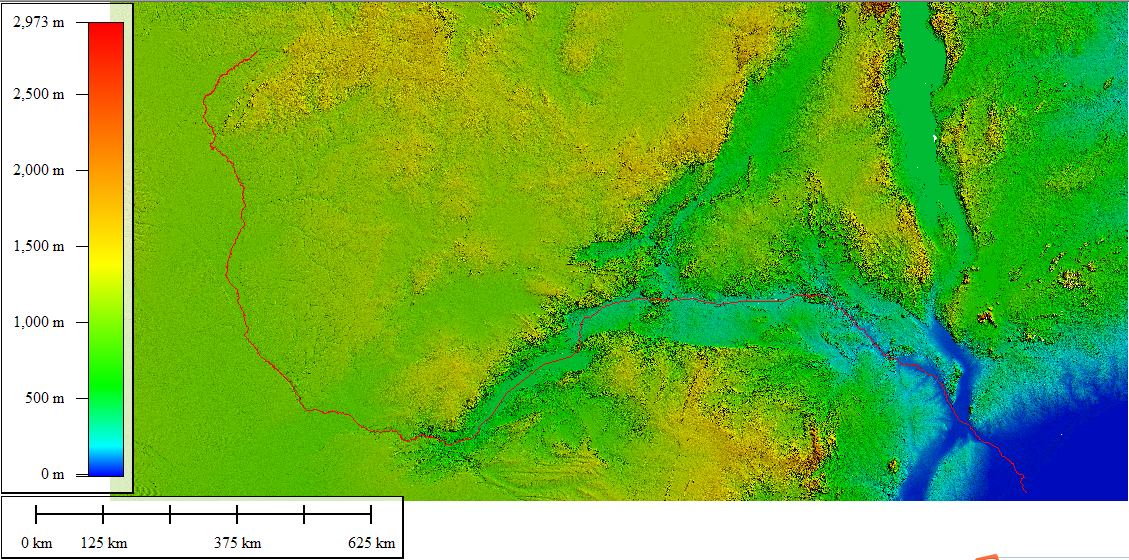
\includegraphics[width=14cm]{./figures/Sensing_Figure.png}
\caption{Overview Elevation Chart} \label{fig:Fig1}
\end{figure}

According to the DEM, we obtain the elevation along the whole Zambezi River. From the Figure 2, the river can be divided into three sections, of which the source goes to the Victoria Falls for the upper reaches, the Victoria Falls to the Cahora Bassa Dam for the middle reaches and the Cahora Bassa Dam to the end for the downstream.

\begin{figure}[h]
\small
\centering
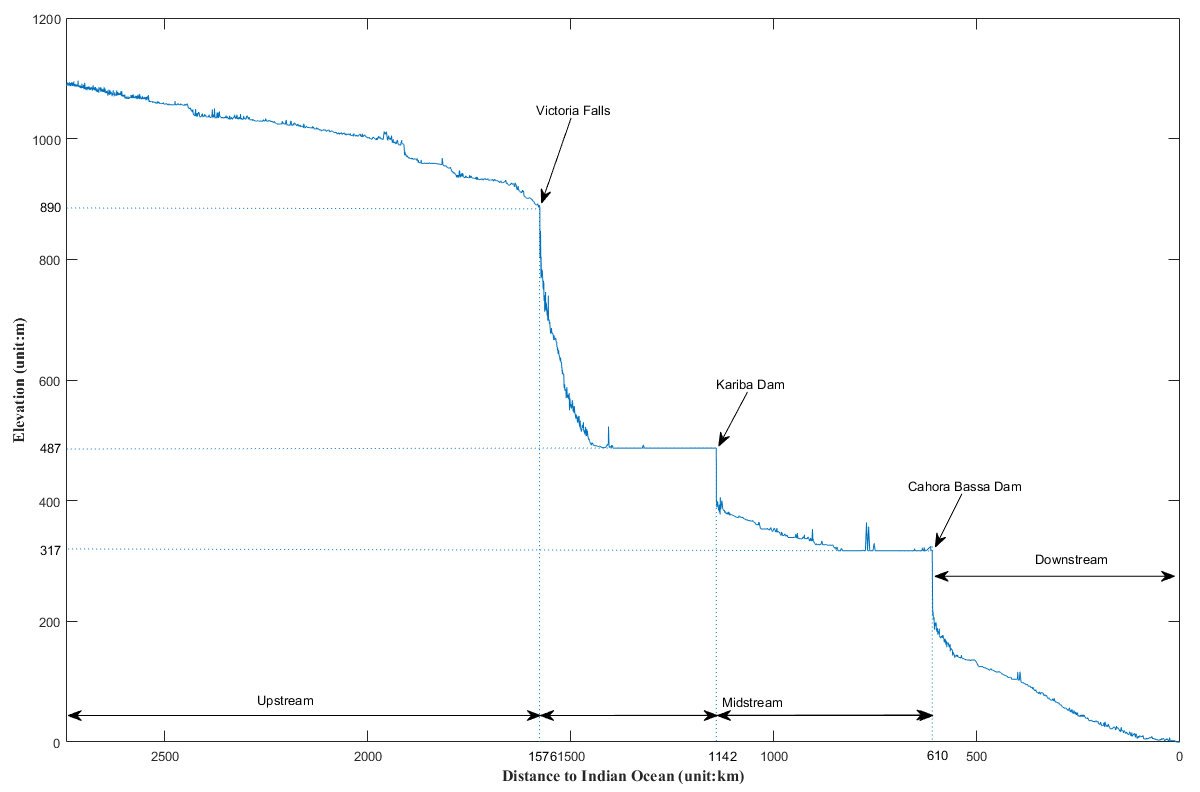
\includegraphics[width=16cm]{./figures/dis_alti_v3.png}
\caption{Elevation along the Zambezi River} \label{fig:Fig2}
\end{figure}

There is a clear trend that the upstream is smooth and have small water level drop, the water level decreases remarkably in the midstream and shoulders the most responsibility of storing water, the downstream have a rapid change of water level as well but there are few dams. Three prominent falls in the water level occur in the Victoria Fall,the Kariba Dam and the Cahora Bassa Dam.

%%%%%%%%%%%%%%%%%attention here!%%%%%%%%%%%%%%%%%%%%%%%%%%
From the perspective of the drop, we know the following areas are suitable for the establishment of dams: a few areas of upstream, reaches between Victoria Fall and Kariba Lake, reaches between Kariba Dam and Cahora Bassa Dam, some areas in the downstream. In addition to the drop, we also need to analyze the slope and height as well as the breadth of the Zambezi River itself for they have great affect on the cost of dam construction. We plotted the contours of the Zambezi River basin based on the DEM model above. Generally, for the sake of storage capacity, safety and ecological impact, the surrounding mountain of the reservoir should be steep as possible and have suitable height. The steepness of the mountain means less area flooded, little 


\subsection{Model Validation}

\subsection{Result}
\indent \indent According to Model A, We get some important equations as follow.

Meanwhile, based on the model, we make the following suggestions.
\begin{itemize}
  \item 
\end{itemize}


\section{Model B : The Best Arrangement}
\subsection{Description}
\subsection{Analysis and Assumptions}
\subsection{Model Building}
\subsection{Optimization}
\subsection{Sensitivity Analysis}
\subsection{Model Validation}
\subsection{Result}




% \section{Analysis of the Problem}
% \begin{figure}[h]
% \small
% \centering
% 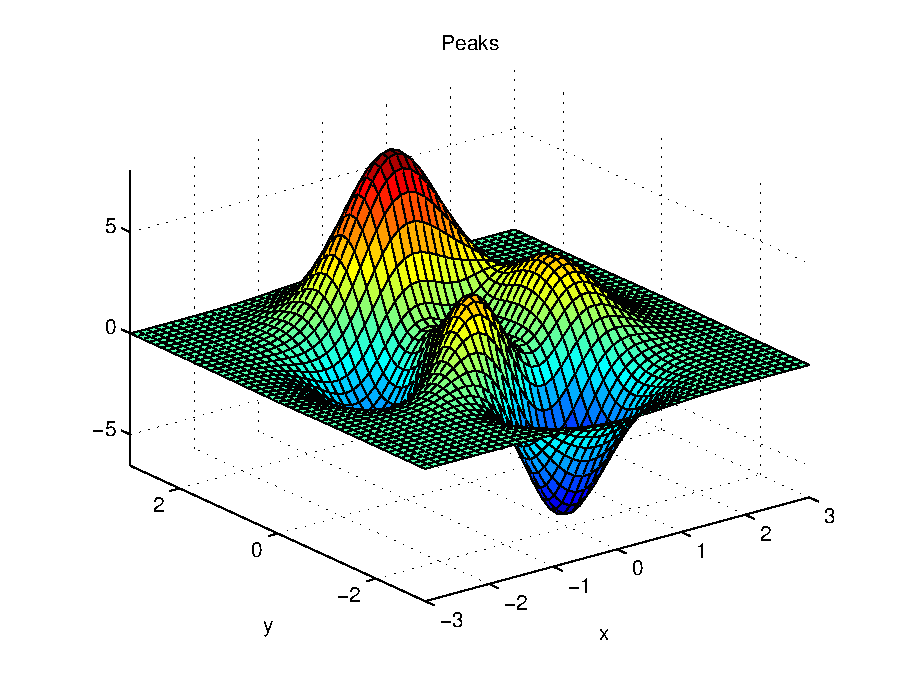
\includegraphics[width=12cm]{mcmthesis-aaa.eps}
% \caption{aa} \label{fig:aa}
% \end{figure}

% \lipsum[8] \eqref{aa}
% \begin{equation}
% a^2 \label{aa}
% \end{equation}

% \[
%   \begin{pmatrix}{*{20}c}
%   {a_{11} } & {a_{12} } & {a_{13} }  \\
%   {a_{21} } & {a_{22} } & {a_{23} }  \\
%   {a_{31} } & {a_{32} } & {a_{33} }  \\
%   \end{pmatrix}
%   = \frac{{Opposite}}{{Hypotenuse}}\cos ^{ - 1} \theta \arcsin \theta
% \]
% \lipsum[9]

% \[
%   p_{j}=\begin{cases} 0,&\text{if $j$ is odd}\\
%   r!\,(-1)^{j/2},&\text{if $j$ is even}
%   \end{cases}
% \]

% \lipsum[10]

% \[
%   \arcsin \theta  =
%   \mathop{{\int\!\!\!\!\!\int\!\!\!\!\!\int}\mkern-31.2mu
%   \bigodot}\limits_\varphi
%   {\mathop {\lim }\limits_{x \to \infty } \frac{{n!}}{{r!\left( {n - r}
%   \right)!}}} \eqno (1)
% \]

\section{Strengths and weaknesses}
\subsection{Model A: Search for possible locations to build dams}
Model A has the following weaknesses.
\begin{itemize}
\item 
\item 
\end{itemize}
Despite of the weakness, it has more strengths.
\begin{itemize}
  \item 
  \item 
\end{itemize}

\subsection{Model B: The Best Arrangement}
In Model B, we consider .... , which is a weakness. However we have more strengths as below:
\begin{itemize}
  \item 
\end{itemize}

\section{Conclusion}
\indent \indent Here is the conclusion to be done!

\begin{thebibliography}{99}
\bibitem{1} IRMSA , Impact of the failure of the Kariba Dam, June 2015.
\bibitem{2}Lamport, Leslie,  \LaTeX{}: `` A Document Preparation System '',
Addison-Wesley Publishing Company, 1986.
\bibitem{3}\url{http://www.latexstudio.net/}
\bibitem{4}\url{http://www.chinatex.org/}
\end{thebibliography}

\clearpage
\section{Brief Assessment of the options}
\indent \indent The solution to the Kariba Dam problem can simply be divided into three options: repairing it, rebuilding it or removing it then replacing it with other dams. To the third method, ZRA suggests to build $10\sim20$ small dams to replace the huge Kariba Dam.\\
\indent Evaluating the options from the perspective of cost and benefit is a complex task, since it can be influence by a number of factors. Only considering the cost of building dams, although it can be estimated accurately by using the cost formula below \\
\[
C_{p} = K\left(\frac{V}{\left(\frac{H}{0.3}\right)^{0.3}}\right)^{0.82}
\]
where $C_{p}$ is the cost of building the hydropower station, $V$ is the installed capacity, $H$ is the design head, $K$ is the proportional coefficient. However, the ecological costs of dam construction need to be considered more cautiously because damage to the ecological environment may be irreversible.\\
\indent Option 1. Repairing the existing Kariba Dam. This is the option with the lowest cost of construction. Meanwhile, it won't change the submerged area, so there is no extra ecological cost. From the aspect of revenue, the reconstruction and expansion of Kariba Dam hydropower station can be carried out at the same time, which can effectively increase the total installed capacity of hydropower station, and thus improve the income of hydropower station. In fact, the expansion of the Kariba Dam hydropower station is underway. Since the reconstruction will not affect the Kariba Lake, the benefits from the use of water from the lake won't be reduced. The analysis above is based on the assumption that the climate will not change drastically in the future and no rare disasters which is outside the historical statistics will occur.\\
\indent Option 2. Rebuilding the existing Kariba Dam. Because rebuilding the Kariba Dam need to remove the existing the dam and rebuild it at the origin site, it is an option with high risk and cost. What's more, the reconstruction of the dam will inevitably lead to the result that the hydropower station can't generate electricity in quite a long period, so this part of loss should also be included in the cost of reconstruction. However, rebuilding dams do have benefits. It helps to expand the installed capacity of hydropower station (benefit from re-designing the internal structure and using more advanced equipment). The new designed Dam would have better flood protection capacity, which allows river management to handle emergency with more flexibility. Stronger water storage capacity means we can raise the water level of Kariba Lake. It will increase the energy generation as well as bring the risk of ecologic damage which needs to be treated with caution.\\
\indent Option 3. Removing the Kariba Dam and replacing it with a series of $10\sim20$ smaller dams along the Zambezi River. This is quite an ambitious plan. Even if the sum of installed capacity of all these small dams is the same as that of Kariba Dam, the total construction cost is still expected to be higher than rebuilding Kariba Dam according to the cost formula above. With the same problem as option 2, removing Kariba Dam will definitely lead to the loss of energy generation, furthermore even the construction of a smaller dam in the original position of Kariba Dam may result in loss of water storage capacity, as the water level in Kariba Lake will decrease. Fortunately, these losses can be minimized through rational planning. Specifically, we can give priority to the construction of small dams, and then gradually replace the Kariba Dam with their power generation capacity. New dams built in the down stream would store the water from Kariba Dam when it is removed, which can reduce the loss of water resources. Different from the previous two options, economic compensation of the new reservoirs' reserved area also needs to be include in the cost.(Here we can make an estimate by calculating the unit area GDP of the catchment)From the ecological point of view, the third option is also accompanied by greater risk. It will not only flood new areas, but also affect the ecology of Lake Kariba (the water level drops and the lake is divided into several parts). In terms of revenue, the scheduling of water resources between dams will reduce the loss of water resources caused by flooding discharge, which will actually help to increase the power generation capacity of hydropower stations. Moreover, the rational allocation of flood storage between dams will increase the safety of the dam system, the reduced reservoir area will reduce the evaporation loss of water and, in the face of emergencies, river management can also adopt a more flexible approach. Because of the high cost of the third option, a long-term analysis is of great significance. In the future, the flow of Zambezi River may reduce by $40\%\sim50\%$ due to the climate change. Although the climate predictions nowadays are with a large degree of uncertainty, but we should never be blindly optimistic about the benefits of the new dam system.\\




% \clearpage
% \begin{appendices}

% \section{First appendix}

% \lipsum[13]

% Here are simulation programs we used in our model as follow.\\

% \textbf{\textcolor[rgb]{0.98,0.00,0.00}{Input matlab source:}}
% \lstinputlisting[language=Matlab]{./code/mcmthesis-matlab1.m}

% \section{Second appendix}

% some more text \textcolor[rgb]{0.98,0.00,0.00}{\textbf{Input C++ source:}}
% \lstinputlisting[language=C++]{./code/mcmthesis-sudoku.cpp}

% \end{appendices}

\end{document}

%%
%% This work consists of these files mcmthesis.dtx,
%%                                   figures/ and
%%                                   code/,
%% and the derived files             mcmthesis.cls,
%%                                   mcmthesis-demo.tex,
%%                                   README,
%%                                   LICENSE,
%%                                   mcmthesis.pdf and
%%                                   mcmthesis-demo.pdf.
%%
%% End of file `mcmthesis-demo.tex'.